\documentclass[11pt]{scrartcl}
%\documentclass[11pt, twoside, a4paper, BCOR8mm, DIV12, bibtotoc,idxtotoc]{scrbook}
%\documentclass[11pt, twoside, a4paper, BCOR8mm, DIV12, bibtotoc,idxtotoc]{scrbook}
\usepackage{german}
\usepackage{path}
\usepackage{typearea}
\usepackage[utf8]{inputenc}
\usepackage{longtable}
\usepackage{hyperref}
\usepackage{graphicx}

% Zusaetzliche Picture-Umgebungen (z.B. shadowenv)
\usepackage{picins}

% Header anpassbar
\usepackage{fancyhdr}

% Headings umdefinieren
\pagestyle{fancy}
\fancyhf{}
\fancyhead[L]{\nouppercase{\rightmark}}
\fancyhead[R]{\thepage}
\fancyfoot[L]{\scriptsize O. Flimm, Die Open-Source-Software OpenBib an der USB Köln - Überblick und Entwicklungen in Richtung OPAC 2.0\newline \textbf{in:} \emph{BIBLIOTHEK. Forschung und Praxis, Jg. 31 (2007) Nr. 2 (c) K. G. Saur Verlag.}}
\parindent0.0mm
\parskip0.3cm    
\typearea{12}

\addtolength{\headheight}{7mm}
\addtolength{\headwidth}{1cm}

\addtolength{\oddsidemargin}{11mm}
\addtolength{\evensidemargin}{-11mm}

\title{Die Open-Source-Software OpenBib an der USB Köln - Überblick und Entwicklungen in Richtung OPAC 2.0}

\author{Oliver Flimm \texttt{<flimm@ub.uni-koeln.de>}}

\date{13.4.2007}
\begin{document}

\begin{titlepage}
\maketitle
\thispagestyle{empty}

\begin{abstract}
  Dieser Artikel beschreibt die vom Autor entwickelte und an der
  Universitäts- und Stadtbibliothek Köln (USB) seit 1997 in
  verschiedenen Projekten eingesetzte Open-Source-Portalsoftware
  OpenBib. Nach einem grundlegenden Einblick in die Ursprünge, Technik
  und konkreten Einsatzgebiete an der USB werden weitergehende
  Funktionen des Portals erläutert, wie RSS-Feeds, Mashups, Tagging,
  Tag-Clouds, Nutzungsanalysen, Drilldowns sowie Kataloganreicherung.
  Viele davon sind charakteristisch für einen OPAC 2.0.
\end{abstract}

\textbf{\fontfamily{cmss}\fontseries{bx}\fontshape{n}\fontsize{12}{12pt}\selectfont The Open Source software OpenBib at the University Library of Cologne (USB) - General overview and developments towards OPAC 2.0}

\begin{abstract}
  This article describes the Open Source portal software OpenBib, a
  project that was started by the author in 1997 and is being used in
  different projects at the University Library of Cologne (USB). After
  a basic overview of the origins, technology and the application at
  the USB the article describes some additional features such as RSS
  feeds, mashups, tagging, tag clouds, use analyses, drilldowns as
  well as catalogue enrichment. Many of these are characteristic for
  OPAC 2.0.
\end{abstract}

\textbf{\fontfamily{cmss}\fontseries{bx}\fontshape{n}\fontsize{12}{12pt}\selectfont
  Le logiciel Open Source OpenBib à la Bibliothèque de l'Université de Cologne (USB) - Vue d'ensemble et développements vers la direction d'un OPAC 2.0}

\begin{abstract}
Cet article décrit le logiciel de portail Open Source OpenBib,
développé par l'auteur et utilisé à la Bibliothèque de l'Université de
Cologne (USB) depuis 1997 en différents projets. Après un regard
élémentaire vers les origines, la technique et les domaines
d'application concrets à l'USB, des fonctions additionelles du portail
sont décrites, comme des flux RSS, des mashups, l'utilisation des
étiquettes, des nuages de mots-clés, des analyses d'utilisation, des
drilldowns ainsi qu'un enrichissement du catalogue. Beaucoup d'en sont
caractéristi\-ques pour un OPAC 2.0.
\end{abstract}

\scriptsize O. Flimm, Die Open-Source-Software OpenBib an der USB Köln - Überblick und Entwicklungen in Richtung OPAC 2.0\newline \textbf{in:} \emph{BIBLIOTHEK. Forschung und Praxis, Jg. 31 (2007) Nr. 2 (c) K. G. Saur Verlag.}
\end{titlepage}

\tableofcontents
\section{KUG und OpenBib}
Die Entwicklung des OpenBib Recherche-Portals\footnote{OpenBib - Das
  OpenSource Recherche-Portal.\newline\path|http://www.openbib.org/|
  (Zugriff am 30.3.2007)} ist eng mit dem IGK-Projekt
(InstitutsGesamtKatalog) verknüpft, das Anfang der 90er Jahre an der
Universitäts- und Stadtbibliothek Köln (USB Köln) angesiedelt wurde
und dessen Nachfolger KUG (Kölner
UniversitätsGesamtkatalog\footnote{KUG - Kölner
  UniversitätsGesamtkatalog.\newline\path|http://kug.ub.uni-koeln.de/|
  (Zugriff am 30.3.2007)}), der 2002 an den Start ging. Vorrangiges
Ziel der Projekte war die Schaffung eines universitätsweiten
bibliothekarischen Gesamtkataloges, bestehend aus den Daten der USB,
der Zentralbibliothek für Medizin (ZB MED) sowie der mehr als 140
Institute bzw. Seminare an der Universität zu Köln, und damit die
Umsetzung der Vorgabe des Ministeriums für Wissenschaft und Forschung
des Landes Nordrhein-Westfalen nach "`funktionaler Einschichtigkeit in
zweischichtigen Bibliothekssystemen"'. Derzeit stellt das an der USB
Köln eingesetzte KUG Recherche-Portal (kurz "`KUG"', Abb. \ref{bild:kug}) den
primären Einsatzort von OpenBib dar.

\begin{shadowenv}
  \vspace{4mm}
    \centering \begin{minipage}[b]{1.0\textwidth}
      \centering 
\includegraphics[width=15cm]{openbib-bfp-2007_bilder/Abb-01-kug-portal.png}
    \end{minipage}
    \caption{Das KUG Recherche-Portal mit mehr als 130 Katalogen als
      primärer Einsatzort von OpenBib}
  \label{bild:kug}
  \vspace{3mm}
\end{shadowenv}

Eine grundlegende Anforderung war von Beginn an die Integration vieler
einzelner Kataloge unter einer einheitlichen Suchoberfläche. Waren die
Kataloge im Instituts- und Seminarbereich zunächst noch über
verschiedene Bibliothekssysteme -- u.a. BISLOK, Allegro, Lars, Lidos,
FileMaker -- verteilt, fand mit dem KUG-Projekt eine Konsolidierung
auf das einheitliche integrierte Bibliothekssystem SISIS-SunRise der
Firma OCLC PICA mit seinen Modulen Katalogisierung, Ausleihe und
Erwerbung statt, das bereits bei der USB und der ZB MED im Einsatz
war. Das System wird auf einem zentralen Datenbankserver betrieben,
auf dem die Bestände eines jeden Instituts in eigenen Datenbanken
gekapselt sind. Neben Katalogdaten aus SISIS-SunRise sind in das
Portal weitere Katalog- und Datenquellen integriert -- u.a. EconBiz und
OAI-Repositories wie der Hochschulschriftenserver der Universität zu
Köln.

Die Präsentation sehr vieler heterogener Daten und die sukzessiv
gemachten Erfahrungen seit Anfang der 90er Jahre haben viele
Design-Entscheidungen bei der Entwicklung von OpenBib maßgeblich
beeinflusst. Es stehen nicht primär Funktionalitäten eines einzelnen
Kataloges im Vordergrund, sondern vielmehr die Erschließung von
Funktionalitäten für die Gesamtheit \emph{aller} Kataloge und Datenbanken.
Sehr oft ist damit ein Abwägungsprozess verbunden -- wie z.B. bei der
Anreicherung der Kataloge mit digitalisierten Inhaltsverzeichnissen
(s.u.) -- bei dem zugunsten eines maximalen Nutzens für alle Kataloge
entschieden wird anstelle minimaler Vorteile für einen einzelnen
Katalog.

\subsection{Entkopplung von Portal und Bibliothekssystemen}
Ein Grundstein für die erfolgreiche Umsetzung der Anforderungen des
KUG-Projektes mit OpenBib ist eine vollständige Entkopplung der
Katalogdaten im Portal von den Ursprungssystemen. Die Voraussetzung
dazu ist der Vollzugriff auf die Daten aller Kataloge, was im
KUG-Projekt von Anfang an gegeben war.

Auf einem Portal-Server sind jeweils die bibliographischen Daten aller
Kataloge in getrennten SQL-Datenbanken abgelegt - einem Katalog aus
einem (theoretisch beliebigen) Ursprungs-Bibliothekssystem entspricht
somit immer eine 'lokale' Datenbank auf allen Portal-Servern. Jeder
Portal-Server umfasst also immer alle Katalogdaten und ist
diesbezüglich autonom. Die nächtliche Synchronisation der Katalogdaten
auf den Portal-Servern mit den Ursprungssystemen geschieht voll
automatisiert. Darüber hinaus verfügt jede Datenbank über einen
eigenständigen Suchmaschinen-Index, der alternativ für
Rechercheanfragen oder Treffermengenanalysen herangezogen werden kann.

Eine direkte Kopplung des Recherche-Portals ist lediglich zur
Ausleih-Komponente der jeweiligen Bibliothekssysteme notwendig -- im
Wesentlichen zur sekundengenauen Ermittlung des Ausleihstatus, zur
Authentifizierung und zur Anzeige der Benutzerkonten. Diese Verbindung
wird über SOAP-basierte WebServices realisiert.

Folgende Vorteile sind mit der Entkopplung der bibliographischen Daten
von den Ursprungssystemen verbunden:
\begin{itemize}
\item Die Ursprungs-Bibliothekssysteme werden von Rechercheanfragen
  entlastet. Bei Wartungsarbeiten und Software-Upgrades der
  Bibliothekssysteme ist weiterhin eine Recherche über das Portal
  möglich.
\item Durch eine "`intelligente"' Lastverteilung zwischen
  verschiedenen Portal-Servern wird das Portal sehr skalierbar.
  Etwaige Performance-Engpässe, z.B. verursacht durch kontinuierlich
  steigende Rechercheanfragen, können sehr schnell durch Hinzunahme
  eines neuen Servers gelöst werden.
\item Die Katalogdaten werden auf den Portal-Servern mit einer fest
  definierten Struktur in den Datenbanken abgelegt. Damit verfügt das
  Portal über eine einheitliche Datenbasis, auf deren Grundlage neue
  Dienste und Funktionen realisiert werden können, die in keinem der
  Usprungssysteme oder nur vereinzelt existieren.
\end{itemize}

Der Zugriff auf eine einheitliche Datenbasis ist eine zentrale
Voraussetzung dafür, dass in einem Recherche-Portal wie dem KUG mit
seinen mehr als 130 Datenbanken und über 5.2 Mio. Titeln in einem
größeren Maßstab durch neue Funktionen ein Mehrwert für den Nutzer
geschaffen wird.

Hier unterscheidet sich OpenBib mit seiner eigenen Datenhaltung
grundsätzlich von herkömmlichen Recherche-Portalen, die Anfragen
lediglich über standardisierte Protokolle wie Z39.50 an verschiedene
Zielsysteme weiterleiten und die gelieferten Ergebnisse präsentieren.
Bei diesen Portalen besteht eine sehr große Abhängigkeit von den zum
Teil höchst unterschiedlichen Fähigkeiten der abgefragen entfernten
Systeme, die damit eine wesentliche Begrenzung darstellen. OpenBib ist
aber nicht das einzige Portal, das von einheitlich abgelegten Daten
profitiert. Ein anderes Beispiel ist der innovative
Dreiländerkatalog\footnote{Dreiländerkatalog.\newline\path|http://suchen.hbz-nrw.de/|
  (Zugriff am 30.3.2007)} des hbz, der komplett auf
Suchmaschinen-Technologie basiert und mit dem Konzept des
Suchraumes\footnote{hbz:
  Suchraum.\newline\path|http://www.hbz-nrw.de/angebote/suchraum/|
  (Zugriff am 30.3.2007)} auf einen Suchindex zugreift.


\subsection{Flexibilität durch Open-Source-Software}
Ein zweiter Grundstein für den Projekt-Erfolg ist eine größtmögliche
Flexibilität bei der Implementierung neuer Funktionen. Zu deren
Realisierung ist ein vollständiger Zugriff auf alle technischen
Komponenten des Portals und deren Änderung bzw. Erweiterung zwingend
notwendig.

Diese Anforderungen werden nur durch den Einsatz von
Open-Source-Komponenten erfüllt, bei denen definitionsgemäß -- im
Gegensatz zu kommerzieller Standardsoftware -- ein vollständiger
Zugriff auf den Quell-Code möglich ist. Erst mit dieser vollständigen
Kontrolle über die Software wird eine sehr schnelle Reaktion auf
Trends und neue Technologien ermöglicht -- dies im Übrigen auch noch
kostengünstig.

Aufgrund dieser Flexibilität lassen sich Projekte sehr schnell
umsetzen. Ein gutes Beispiel hierfür ist die "`Digitale Einbandsammlung
der USB Köln"', die von der ersten Konzeption bis zur finalen
Umsetzung nur wenige Monate benötigte\footnote{Vgl.  Regine Boeff,
  Oliver Flimm: Von der traditionellen zur digitalen Sammlung
  historischer und künstlerischer Bucheinbände der USB Köln mit einem
  Einblick in die technische Konzeption der Datenbank ; in:
  Bibliothek. Forschung und Praxis. Jahrgang 30 (2006) Nr. 1,
  S.63--68}.

Der Einsatz von Open-Source-Software am Beispiel von OpenBib hat sich
auch im Produktionsbetrieb im Vergleich zu kommerzieller
Standardsoftware als sehr vorteilhaft erwiesen:
\begin{itemize}
\item Erweiterungen werden umgehend selbständig vorgenommen und
  Probleme in der Regel deutlich schneller gelöst.
\item Von unseren Benutzern an uns herangetragene Wünsche werden
  ebenfalls schneller umgesetzt.
\item Release-Zyklen der Software werden selbst vorgegeben.
\item Die Integration von anderen Software-Produkten über
  standardisierte Schnittstellen ist mit wenig Aufwand möglich.
\end{itemize}

\section{Ursprung und Technik von OpenBib}
Die Portalsoftware OpenBib ist seit ihrer ersten Version aus dem Jahr
1997, in der sie als "`Freizeitprojekt"' begonnen wurde und historisch
noch unter dem Namen 'biblio' firmierte, als Open-Source-Software
verfügbar. Als Garant für die Freiheit\footnote{Free Software
  Foundation (FSF) / GNU Project: The Free Software
  Definition.\newline\path|http://www.gnu.org/philosophy/free-sw.html|
  (Zugriff am 30.3.2007)} dieser Software und gegen unerwünschte
kommerzielle Vereinnahmung wurde bewusst die schon bei Linux
verwendete GNU General Public License (GPL) gewählt. Schon wenig
später -- im Oktober 1997 -- wurde biblio/OpenBib von der USB zur
Realisierung des KVIK (Kölner Virtueller
InstitutsgesamtKatalog\footnote{Kölner Virtueller
  InstitutsgesamtKatalog.\newline\path|http://kvik.ub.uni-koeln.de/|
  (Zugriff am 30.3.2007)}, dem Vorgänger des KUG) genutzt, mit zuletzt
knapp 750.000 Titeln in 74 Katalogen im Juni 2002.

OpenBib basiert seinerseits wieder auf verbreiteten
Open-Source-Komponenten -- speziell Linux, Apache, MySQL und
Perl. Damit handelt es sich um ein typisches LAMP-System mit einer
niedrigen Einstiegsschwelle für einen erfahrenen LAMP-Entwickler.

Von ihrer ersten Version entwickelte sich die Software von einer
reinen Sammlung an CGI-Skripten mit wenigen mod\_perl-Elementen aus den
Jahren 1997-2004 zu einer vollständig mod\_perl-ba\-sier\-ten, direkt in
den Apache-Webserver integrierten Webanwendung. In dieser Webanwendung
wird zusammen mit den zugrunde liegenden Datenbanken sowie einem
Tem\-pla\-ting-System (Perl Template Toolkit) das sog. MVC-Design-Pattern
realisiert und damit speziell die sinnvolle Trennung von
Programm-Logik und Darstellung. Dadurch lassen sich auch sehr gut die
entsprechenden Zuständigkeiten für Programmierung und Web-Design an
verschiedene Mitarbeiter verteilen.

\subsection{Kaskadierung von Templates, CSS und Texten} 
Durch die Verwendung der Templates können die Web-Oberflächen
differenziert dargestellt und mit geringem Aufwand angepasst
werden. Um den Aufwand für den Betrieb sehr vieler visuell
eigenständiger Portal-Sichten zu minimieren, lassen sich die Templates
katalog- und sichtspezifisch kaskadieren. Für eine einzelne
Katalogsicht müssen damit nicht jeweils alle Templates für jede Sicht
getrennt verwaltet, sondern lediglich die geänderten Templates an fest
definierten Stellen abgelegt werden. Vor der Ausgabe eines Templates
wird zunächst überprüft, ob es ein spezielles Template für diesen
Katalog oder diese Sicht gibt -- und dieses gegebenenfalls
verwendet. Falls nicht, kommt das zugehörige Standard-Template zur
Anwendung.

Wie bei den Templates lassen sich durch einen ähnlichen Mechanismus
auch Cascading Stylesheets (CSS) und auszugebende Texte katalog- und
sichtspezifisch kaskadieren. Die Möglichkeit, in Abhängigkeit vom
Katalog andere Texte für identische Katalogkategorien zu vergeben,
wird im KUG ausgiebig für Spezialkataloge mit alternativen
Kategorienamen genutzt, wie der Einbandsammlung und der
Portraitsammlung. So tritt bei der Portraitsammlung beispielsweise die
Bezeichnung 'Maler, Zeichner' an die Stelle von 'Verfasser' in der
MAB2-Kategorie 100.

Im KUG werden mit diesen einfachen Kaskadierungs-Techniken ausgehend
von einfachen Institutssichten bis hin zu aufwändigeren Fach-Portalen
insgesamt 144 unterschiedliche Portal-Versionen im Rahmen nur einer
OpenBib-Softwareinstallation angeboten.

\subsection{Recherche-Backends, UTF8-Encoding und I18N} 
Für die Suche im Portal stehen zwei alternative Recherche-Backends zur
Verfügung. Neben einer klassischen Recherche über SQL kann auch ein
Suchmaschinen-Backend verwendet werden. Dieses bietet weitergehende
Möglichkeiten wie z.B. Treffermengen- sowie Termanalysen und basiert
auf der Open-Source-Suchmaschinentechnologie von Xapian\footnote{The
  Xapian Project.\newline\path|http://www.xapian.org/| (Zugriff am
  30.3.2007)}.

Im KUG wird der Suchmaschinen-Index für die "`Einfache Recherche"' und
das SQL-Backend für die "`Komplexe Recherche"' verwendet. Während das
Suchmaschinen-Backend gerade bei alltäglichen Suchanfragen, wie sie
von einem Großteil der Recherchierenden gestellt werden, seine Stärken
auspielt, ist diese Technologie weniger für sehr spezialisierte
Recherche-Anfor\-de\-run\-gen geeignet, wie sie z.B. aus dem
bibliothekarischen Bereich unserer Nutzer gefordert werden. Deren
Anforderungen können nur durch das SQL-Backend erfüllt werden.

Die Datenbankstruktur für die Katalogdaten ist sehr flexibel. MAB2
wird standardmäßig als Format sowohl in den SQL-Datenbanken wie auch
für die vereinheitlichten Meta-Daten genutzt. Grundsätzlich sind aber
auch andere Kategorienschemata oder Meta-Datenformate -- wie
z.B. MARC21 -- mit entsprechendem Anpassungsaufwand möglich.

Als Standard-Encoding für das Portal wird zeitgemäß UTF8
verwendet. Damit lassen sich auch Katalog-Bestände aus UTF8-fähigen
Bibliothekssystemen in das Portal integrieren.

Mit der Verwendung von GNU gettext kann das Portal grundsätzlich auch
in alternativen Sprachversionen angeboten werden. Derzeit wird der KUG
nur in deutscher Sprache angeboten. Eine Übersetzung in die englische
Sprache wurde bereits begonnen.

\subsection{Administration und Betrieb}
Gerade die Administration von vielen Datenbanken in einem Portal ist
ein sehr wichtiger -- wenn auch für den Endanwender weitgehend
unsichtbarer -- Aspekt beim Betrieb des Portals. Aus diesem Grund
verfügt OpenBib über eine bequeme, web-basierte
Administrations-Oberfläche (Abb. \ref{bild:admin}), die den
Arbeitsaufwand wesentlich minimiert. Neben den Katalogen lassen sich
dort auch die Sichten, RSS-Feeds usw. konfigurieren sowie die aktiven
Sessions überwachen.

Die Anforderungen von OpenBib an die Rechnerausstattung sind
bescheiden. Das KUG Recher\-che-Portal wird lediglich mit drei
Doppel-Pentium-III Servern (1.16 GHz CPU, 4 GB RAM) im RAID-Level 1
aus dem Jahr 2002 betrieben. Mit dieser Ausstattung konnten im Jahr
2006 insgesamt 557.445 Benutzer-Sessions mit mehr als 4 Mio.
Recherche-Anfragen problemlos bewältigt werden, davon knapp 400.000
Anfragen über die Einbindung des KUG in die Digitale Bibliothek NRW
(DigiBib\footnote{Digitale Bibliothek
  (DigiBib).\newline\path|http://www.digibib.net/| (Zugriff am
  30.3.2007)}, s.u.).

Die Infrastruktur für das OpenBib-Projekt\footnote{BerliOS Developer:
  Project Info - OpenBib
  Recherche-Portal.\newline\path|http://developer.berlios.de/projects/openbib/|
  (Zugriff am 30.3.2007)} wird von BerliOS\footnote{BerliOS - The Open
  Source Mediator.\newline\path|http://www.berlios.de/| (Zugriff am
  30.3.2007)} bereitgestellt.  Dort findet auch die ausschließliche
Entwicklung über ein CVS-Repository\footnote{OpenBib CVS-Repository
  bei
  BerliOS.\newline\path|http://cvs.berlios.de/cgi-bin/viewcvs.cgi/openbib/openbib/|
  (Zugriff am 30.3.2007)} statt.

\begin{shadowenv}
  \vspace{4mm}
    \centering \begin{minipage}[b]{1.0\textwidth}
      \centering 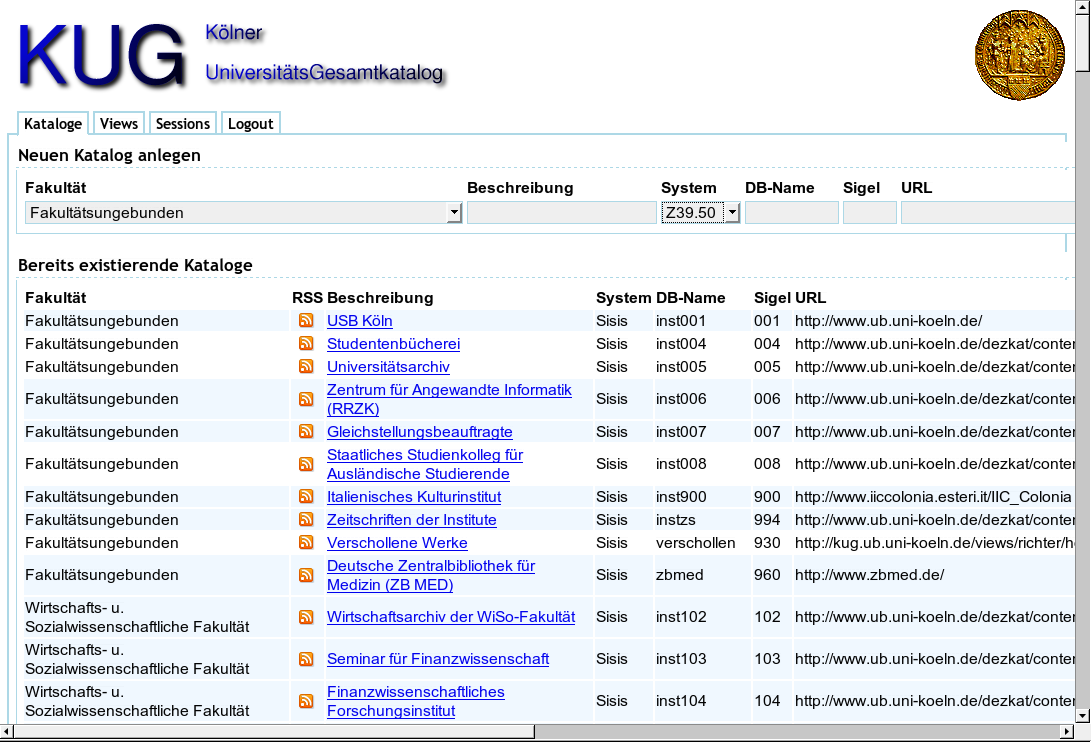
\includegraphics[width=15cm]{openbib-bfp-2007_bilder/Abb-02-administration.png}
    \end{minipage}
    \caption{Die Administrations-Oberfläche des Portals}
  \label{bild:admin}
  \vspace{3mm}
\end{shadowenv}

\section{Einsatz in Fach-Portalen}
Durch die flexiblen Möglichkeiten der Anpassung über eigene Sichten
war die Software des Recherche-Portals predestiniert für den Einsatz
in weiteren Projekten.
 
Hier sind insbesondere die folgenden eigenständigen Fach-Portale zu nennen: 
\begin{itemize}
\item Die Digitale Einbandsammlung der USB Köln\footnote{Digitale
    Einbandsammlung der Universitäts- und Stadtbibliothek
    Köln.\newline\path|http://einbandsammlung.ub.uni-koeln.de/|
    (Zugriff am 30.3.2007)}
\item Die Virtuelle Bibliothek Elise und Helene
  Richter\footnote{Virtuelle Bibliothek Elise und Helene
    Richter.\newline\path|http://richterbibliothek.ub.uni-koeln.de/|
    (Zugriff am 30.7.2007)} als Teil der NS-Provenienzforschung in der
  USB Köln
\item Die Virtuelle Bibliothek Historische Bestände im
  Rheinland\footnote{Virtuelle Bibliothek Historische Bestände im
    Rheinland.\newline\path|http://rheinlandbib.ub.uni-koeln.de/| (Zugriff
    am 30.3.2007)} (Abb. \ref{bild:rheinlandbib})
\item Die Portraitsammlung der USB Köln\footnote{Portraitsammlung der
    Universitäts- und Stadtbibliothek
    Köln.\newline\path|http://portraitsammlung.ub.uni-koeln.de/|
    (Zugriff am 30.3.2007)}
\item Europäische Städte- und Landschaftsbilder des 16. und 17.
  Jahrhunderts\footnote{Europäische Städte- und
    Landschaftsdarstellungen des 16. und 17.
    Jahrhunderts.\newline\path|http://landschaftsbilder.ub.uni-koeln.de/|
    (Zugriff am 30.3.2007)}
\end{itemize}

\begin{shadowenv}
  \vspace{4mm}
    \centering \begin{minipage}[b]{1.0\textwidth}
      \centering 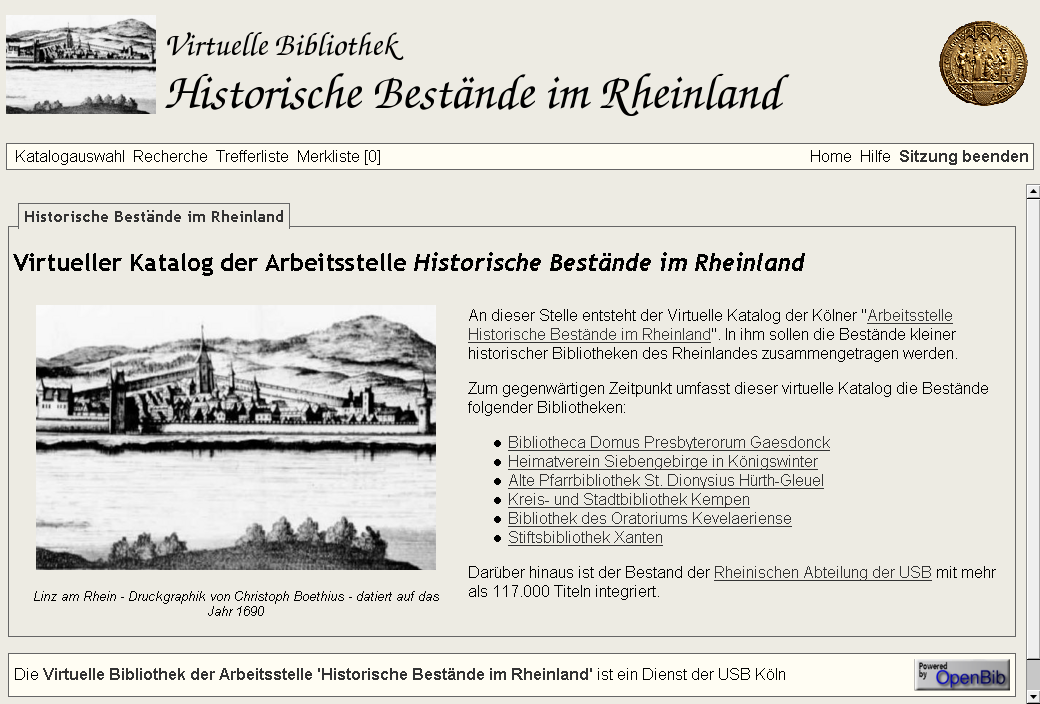
\includegraphics[width=15cm]{openbib-bfp-2007_bilder/Abb-03-rheinlandbib.png}
    \end{minipage}
    \caption{Die Virtuelle Bibliothek 'Historische Bestände im Rheinland' als Beispiel für ein eigenständiges Fach-Portal}
  \label{bild:rheinlandbib}
  \vspace{3mm}
\end{shadowenv}

\section{Anreicherungen, Mashups und OPAC 2.0}
Seitdem Michael Casey im Jahr 2005 den Begriff "`Library 2.0"' in
Anlehnung an das "`Web 2.0"' erstmals erwähnte, wurde verstärkt nach
nutzbringenden Anwendungen von Techniken und Prinzipien des Web 2.0 im
Kontext einer Bibliothek geforscht. Ebenso wird geänderten
Nutzungsgewohnheiten Rechnung getragen, die sich bei den Nutzern
inzwischen durch das Internet und den dort angesiedelten Diensten
(u.a. Amazon und Google) manifestiert haben. Bei allen Überlegungen
werden aktuelle Anforderungen eines Bibliotheksbenutzers an eine
zeitgemäße Bibliothek und ein Mehrwert für ihn in den Mittelpunkt
gestellt. Der OPAC als eine zentrale Bibliotheksanwendung für den
Nutzer rückt im Zuge dieser Verbesserungen als "`OPAC 2.0"' in den
Vordergrund.

Wie andere Kataloge auch, z.B. der innovative XOPAC\footnote{X-OPAC
  Extendable Online Public Access
  Catalog.\newline\path|http://www.xopac.org/| (Zugriff am 30.3.2007)}
aus Karlsruhe, hat der KUG mit OpenBib viele Ideen aufgegriffen und
bereits umgesetzt.  Speziell die Idee des "`sozialen Web"' ist in
einige der aktuellen Entwicklungen eingeflossen.

Die Erweiterungen von OpenBib am Beispiel des KUG lassen sich in
verschiedene Bereiche einordnen:
\begin{itemize}
\item Grundsätzliche Anreicherung der Katalogdaten mit weiteren
  Informationen
  \begin{itemize}
  \item Digitalisierte Inhaltsverzeichnisse
  \end{itemize}
\item Funktionen, die dem Nutzer einen Überblick über Kataloginhalt
  und -nutzung und damit \emph{grobe Orientierungshilfen} bieten
  \begin{itemize}
  \item Tag-Clouds für im Katalog vergebene Schlagworte, Notationen,
    Körperschaften, Personen sowie durch Nutzer vergebene Tags
  \item Popularitäts-Funktion: Top 20 Titel eines Kataloges bezogen
    auf Ausleihe und Nutzung im KUG
  \end{itemize}
\item Funktionen, die aufgrund der Katalogstruktur oder der Analyse
  des Nutzungsverhaltens \emph{direkte Hilfestellungen} in Treffermengen und
  Einzeltrefferansichten anbieten. Das sind u.a.:
  \begin{itemize}
  \item Recommender-Funktion: "`Das könnte Sie interessieren"'
  \item Popularitäts-Funktion: Sortierung nach Popularität
  \item Individuelles und gemeinschaftliches Indexieren ("`Tagging"')
  \item Tag-Clouds für die Verteilung von relevanten Termen in Treffermengen
  \item Drilldowns in Treffermengen
  \end{itemize}
\item Funktionen, die dem Nutzer über Zugriffsschnittstellen oder
  Mashups \emph{weitere Nutzungs\-mög\-lich\-kei\-ten} bieten
  \begin{itemize}
  \item RSS-Feeds für Neuzugänge in den Katalogen
  \item Mashup mit der Social-Software BibSonomy
  \item Mashup mit der Wikipedia für Personen und ISBN-Suche
  \item Mashup mit weiteren Recherche-Portalen
  \end{itemize}
\end{itemize}

Im Folgenden werden einige dieser nutzerzentrierten Funktionen von
OpenBib im KUG näher ausgeführt.

\subsection{Ergebnisanreicherung aller KUG-Datenbanken durch gescannte Inhaltsverzeichnisse}
Unter der Federführung des Hochschulbibliothekszentrums NRW (hbz),
unterstützt vom Ministerium für Innovation, Wissenschaft, Forschung
und Technologie des Landes Nordrhein-Westfalen und durchgeführt von
der Firma ImageWare Components GmbH in Zusammenarbeit mit den
beteiligten Bibliotheken, wurden seit Herbst 2005 an der USB Köln und
der ZB MED im Projekt 180T Inhaltsverzeichnisse von Büchern gescannt
und mit einer OCR-Schrifterkennung bearbeitet (Wirtschafts- u.
Sozialwissenschaften, Medizin). Ziel ist das sog. Catalogue
Enrichment\footnote{hbz: Catalogue
  Enrichment.\newline\path|http://www.hbz-nrw.de/angebote/catalogue\_enrichment/|
  (Zugriff am 30.3.2007)}, also sowohl eine Such- wie auch
Ergebnisanreicherung in Online-Katalogen.

Da dieses Projekt in seiner eigentlichen Konzeption auf die
Anreicherung des USB- bzw. Verbundkataloges ausgerichtet ist, wurde
von uns dieses Konzept lokal für einen Einsatz im Institutsumfeld in
der Form eines allgemeinen Anreicherungskonzeptes für den KUG
erweitert, so dass wir die in diesem Projekt gewonnenen digitalen
Inhaltsverzeichnisse der USB auch für alle Institute und Seminare
nutzbar machen können.

Über eine zentrale Anreicherungsdatenbank können zusätzliche Inhalte
katalogübergreifend in die vorhandenen Katalogdaten eingeblendet oder
für eine Suche herangezogen werden. Grundlage ist eine vorhandene
ISBN.

Diese Einschränkung ist notwendig, wenn ein Nutzen für eine
größtmögliche Anzahl an Katalogen erzielt werden soll. Denn
Anreicherungsinformationen sind nun nicht mehr mit einem speziellen
Titel in einem speziellen Katalog verknüpft, sondern ganz allgemein -- 
und damit automatisch nutzbar für alle Kataloge -- über die ISBN. Der
jeweilige Titel in irgendeinem Katalog "`weiß"' von einer möglichen
Anreicherung nichts. Erst bei der Einzeltrefferanzeige werden für
einen konkreten Titel Katalog- und Anreicherungsdaten kombiniert und
dann ausgegeben.

Bei der Inhaltsanreicherung durch digitalisierte Inhaltsverzeichnisse
bedeutet diese "'portal\-zen\-trier\-te Sichtweise"' im Vergleich zur einer
"`einzelkatalogzentrierten Sichtweise"' im konkreten Fall einen
"`hypothetischen Verlust"' von knapp 9 Prozent an
Inhaltsverzeichnissen für den USB Katalog zugunsten aller anderen.
Dieser Titel-Anteil verfügt über keine ISBN.

Da in den USB Katalog jedoch die Inhaltsverzeichnisse ohnehin über
regelmäßige MAB2-Exporte aus dem Verbundkatalog Einzug finden, sind
auch im USB-Katalog im Kontext des KUG schließlich wieder alle
Inhaltsverzeichnisse zugreifbar.

Wie schon ausgeführt ist die Konzeption der Ergebnisanreicherung in
OpenBib so allgemein gehalten, dass sie sich neben der
Ergebnisanreicherung mit Inhaltsverzeichnissen auch mit anderen
Zusatzinformationen nutzen lässt. So können beliebige Informationen,
wie Nutzer-Reviews, Abstracts, Stichwortverzeichnisse (nach Absprache
mit den entsprechenden Rechteinhabern) u.ä., dort zentral abgelegt
werden und sind für alle Kataloge des OpenBib-Portals automatisch
nutzbar.

\subsection{Individuelles und gemeinschaftliches Indexieren ("`Tagging"')}
Die Indexierung von Dokumenten durch vom Nutzer selbst gewählte
"`Etiketten"' oder Mini-Schlagworte (engl. tags) hat sich im Bereich
sozialer Software -- z.B. in Web 2.0-Diensten wie BibSonomy, flickr
oder del.icio.us -- als ein effektiver Mechanismus bewährt, mit dem
sich
\begin{enumerate}
\item Dokumente individuell organisieren und in Gruppen zusammenfassen
  lassen
\item diese zunächst individuell motivierten Tag-Sammlungen und
  Dokument-Gruppen zum Vorteil anderer Nutzer verwenden lassen
\end{enumerate}

Dieser Mechanismus ist auch auf die Kennzeichnung von Titeln in
Bibliothekskatalogen durch Nutzer übertragbar und deckt dort
verschiedene Bereiche ab: Als "`individuell strukturierbare
Merkliste"', als Alternative zur formalen und inhaltlichen
Sacherschließung durch Bibliothekare\footnote{Dies gilt insbesondere
  dann, wenn keine Sacherschließung mit Schlagworten oder Systematiken
  durch Bibliothekare vorgenommen wird, wie es z.B. bei einigen
  Katalogen im KUG der Fall ist.} sowie als Instrument, um Nutzer auf
weitere thematisch ähnliche Titel aufmerksam zu machen.

\begin{shadowenv}
  \vspace{4mm}
    \centering \begin{minipage}[b]{1.0\textwidth}
      \centering 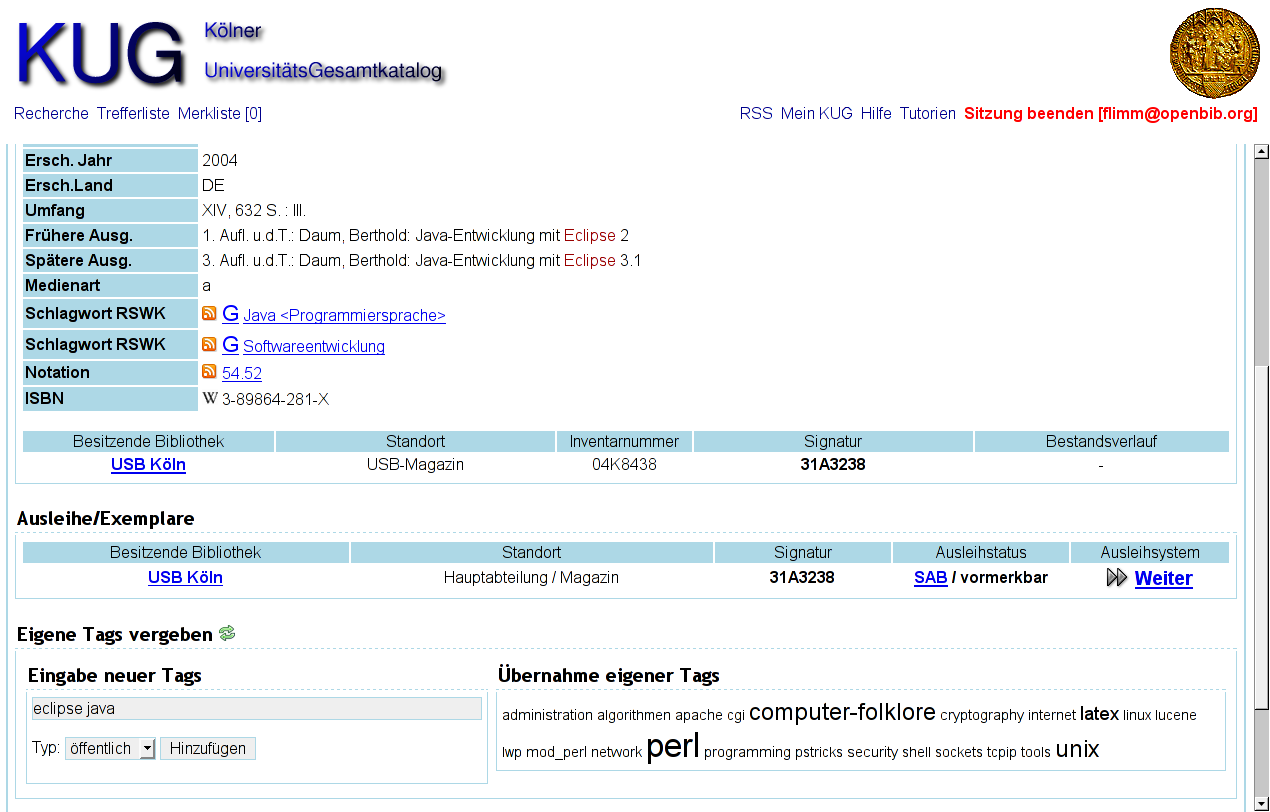
\includegraphics[width=15cm]{openbib-bfp-2007_bilder/Abb-04-tagging.png}
    \end{minipage}
    \caption{Vergabe von Tags für einen Titel}
  \label{bild:tagging}
  \vspace{3mm}
\end{shadowenv}

Von OpenBib wird sowohl individuelles wie auch gemeinschaftliches
Indexieren\footnote{Artikel Gemeinschaftliches Indexieren aus der
  Wikipedia.\newline\path|http://de.wikipedia.org/wiki/Gemeinschaftliches\_Indexieren|
  (Zugriff am 10.4.2007)} unterstützt. Die Vergabe von Tags ist auf am
Portal angemeldete Nutzer beschränkt.

Der bibliothekspolitischen Dimension als Alternative zu der von
Bibliothekaren vorgenommenen Sacherschließung -- "`Soll der Nutzer
überhaupt zum Katalog durch eigene Verschlagwortung beitragen dürfen?
"' -- wird in OpenBib dadurch Rechnung getragen, dass zentral
festgelegt werden kann, ob lediglich individuelles Indexieren in Form
von "`individuell strukturierbaren Merklisten"' oder aber das gesamte
Spektrum des gemeinschaftlichen Indexierens und Nutzens -- also
wirkliches "`Social"'-Tagging -- freigegeben werden soll. Letzteres
ist die Standardeinstellung in OpenBib.

Ein Problem, das beim gemeinschaftlichen, aber auch individuellen
Indexieren auftreten kann, ist die Zersplitterung des "`Tag-Raumes"' 
durch die Verwendung von Umlauten, Groß-Klein\-schrei\-bung und
verschiedenen Wortformen. Aus diesem Grund ist es sehr sinnvoll,
dieser Zersplitterung sowohl durch eine aufgezwungene wie auch
freiwillige Vereinheitlichung von Tags entgegen zu wirken.

OpenBib löst daher bei der Vergabe von Tags zu einem Titel automatisch
Umlaute auf, transformiert in Kleinschreibung und eliminiert
unerwünschte Zeichen in den Tags. Neben diesen aufgezwungenen
Maßnahmen werden dem Nutzer zusätzlich als Orientierungshilfe für die
Tag-Wahl alle von ihm bereits generell vergebenen Tags sowie die von
anderen Nutzern für den konkreten Titel bereits genutzten Tags in Form
von Wortwolken (s.u.) dargestellt. Durch Klick auf einen Tag aus den
Wortwolken wird dieser automatisch in das Eingabefeld eingetragen.
Ferner kann für die Tags eines Titels festgelegt werden, ob diese nur
privat oder auch öffentlich zugänglich sind.

Beim Aufruf eines einzelnen Titels werden alle als öffentlich
definierten Tags zu diesem Titel ausgegeben. Über diese kann jeder
Nutzer auf alle anderen so gekennzeichneten Titel zugreifen. Ist ein
Nutzer am Portal angemeldet, dann werden zusätzlich seine eigenen Tags
dargestellt und ihm darüber der Zugriff auf alle durch ihn damit
verknüpften Titel ermöglicht.

Jenseits der Tags eines einzelnen Titels runden allgemeine Übersichten
eines angemeldeten Nutzers über alle seine Tags und damit Titel sowie
der von allen Nutzern für die jeweiligen Kataloge vergebenen Tags die
Tagging-Funktionen in OpenBib ab.


\subsection{Tag-Clouds als Orientierungshilfe}
Zur Visualisierung von nutzerdefinierten Tags werden diese in vielen
Web 2.0-Diensten als verlinkte "`Wortwolken\footnote{Artikel Wortwolke
  aus der Wikipedia.\newline\path|http://de.wikipedia.org/wiki/Wortwolke|
  (Zugriff am 10.4.2007)}"' (engl. tag cloud) dargestellt. Mit Hilfe
dieser Wolken-Ansicht bekommt der Nutzer eine sehr gute Übersicht der
vergebenen Tags sowie über deren Häufigkeit. Je öfter ein Tag
verwendet wird, desto größer wird es dargestellt.

\begin{shadowenv}
  \vspace{4mm}
    \centering \begin{minipage}[b]{1.0\textwidth}
      \centering 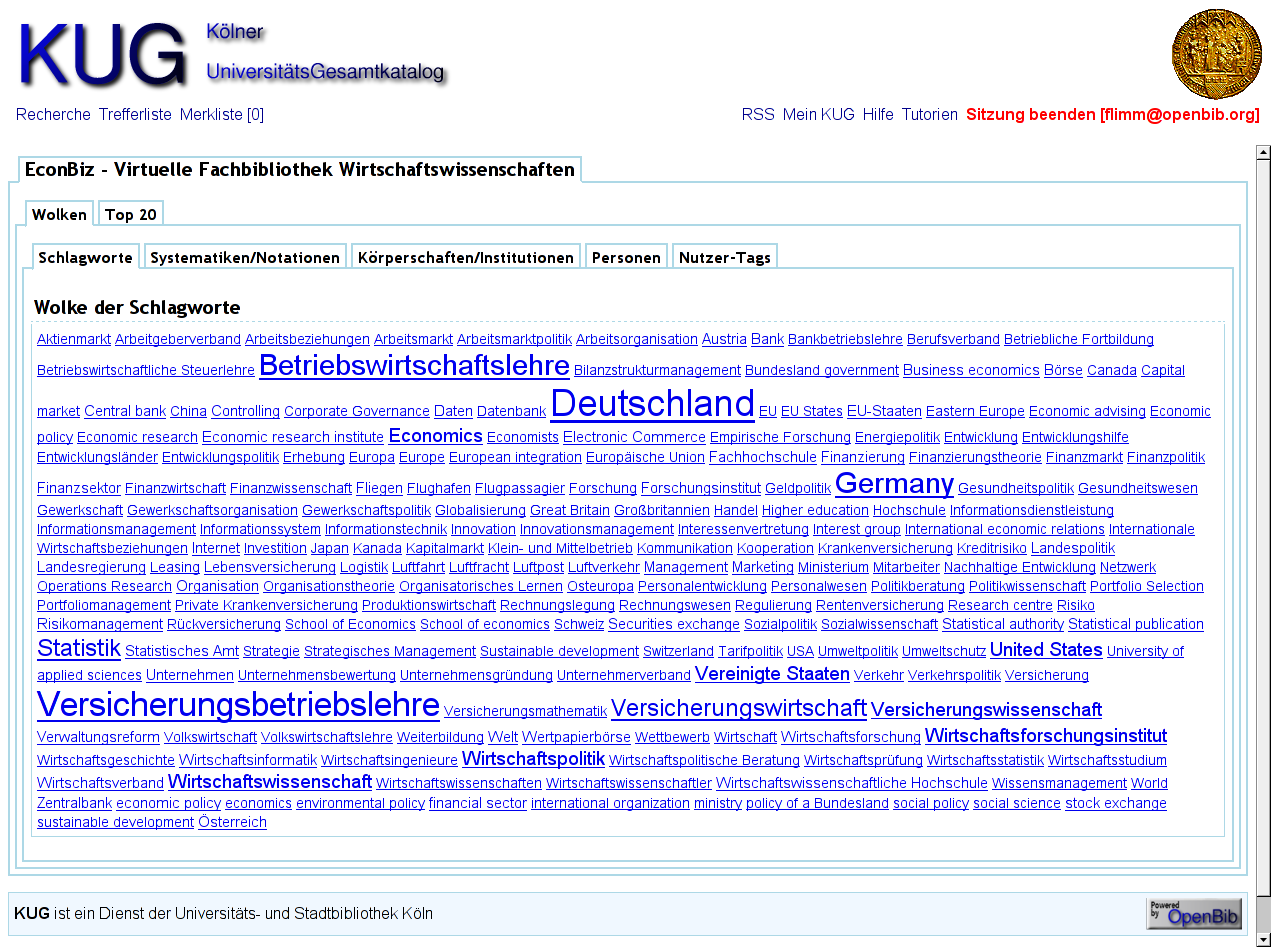
\includegraphics[width=15cm]{openbib-bfp-2007_bilder/Abb-05-schlagwortwolke.png}
    \end{minipage}
    \caption{Der Bestand von EconBiz als Beispiel für eine visuelle Aufschlüsselung nach Schlagworten mit Tag-Clouds}
  \label{bild:tagcloud}
  \vspace{3mm}
\end{shadowenv}


Gerade in einem Bibliothekskatalog ist die vorhande Verschlagwortung
für den Nutzer oft weder durchschaubar noch direkt greifbar. Ob, wie
und in welchem Ausmaß in einem Katalog verschlagwortet wurde,
erschließt sich ihm vielfach nicht.

Hier bieten Wortwolken -- auch an anderen Stellen des Kataloges
jenseits der Schlagworte -- eine elegante Möglichkeit, um dem Nutzer
"`mehr Ein- und Übersicht"' zu bieten. In OpenBib werden solche
"`Übersichts-Wolken"' derzeit an mehreren Stellen eingesetzt.
\begin{enumerate}
\item bei der Verteilung der Schlagworte eines Kataloges, bezogen auf
  die $n$ häufigsten Schlagworte (Standard: $n=200$, Abb. \ref{bild:tagcloud}). Ebenso
  werden auch die anderen Normdaten-Arten, wie Systematik,
  Körperschaften und Personen in Form einer Wortwolke für die
  einzelnen Kataloge dargestellt
\item bei der Verteilung der mit Tags individuell oder
  gemeinschaftlich indexierten Titel (titel-, nutzer- und
  katalog-spezifisch)
\item bei der Verteilung der relevanten Terme, bezogen auf deren
  Häufigkeit in einem Ergebnis-Trefferset und bezogen auf die ersten $n$
  Treffer (Standard: $n=200$)
\end{enumerate}

Weitere Einsatzgebiete sind möglich, wie z.B. der Verteilung der im
Katalog von Nutzern verwendeten Suchbegriffe (Suchwolke). Suchwolken
werden u.a. bereits im kommerziellen Findus
Internet-OPAC\footnote{Findus
  Internet-OPAC.\newline\path|http://www.findus-internet-opac.de/|
  (Zugriff am 30.3.2007)} verwendet, der vorrangig bei Stadt- u.
Gemeindebüchereien eingesetzt wird\footnote{Z.B. Bibliothek Wasserburg
  - Katalog
  (OPAC).\newline\path|http://www.wasserburg.de/de/bibliothek/katalog/|,
  "`Was andere Suchen"' (Zugriff am 1.3.2007)}.

\subsection{Auswertung des Nutzungsverhaltens}
Dienste wie Amazon machen vor, wie eine Analyse des Nutzungsverhaltens
in der Online-Plattform zu einem Mehrwert für den Kunden führen
kann. Entsprechend der zugrunde liegenden Datenbasis aus Verkäufen und
der Auswahl konkreter Produkte für eine Detail-Ansicht, werden für den
Kunden Funktionen wie "`Kunden, die diesen Artikel kauften oder
ansahen, haben auch\dots"' oder "`Die beliebtesten Artikel"' (bezogen
auf eine Recherche) realisiert.

\begin{shadowenv}
  \vspace{4mm}
    \centering \begin{minipage}[b]{1.0\textwidth}
      \centering 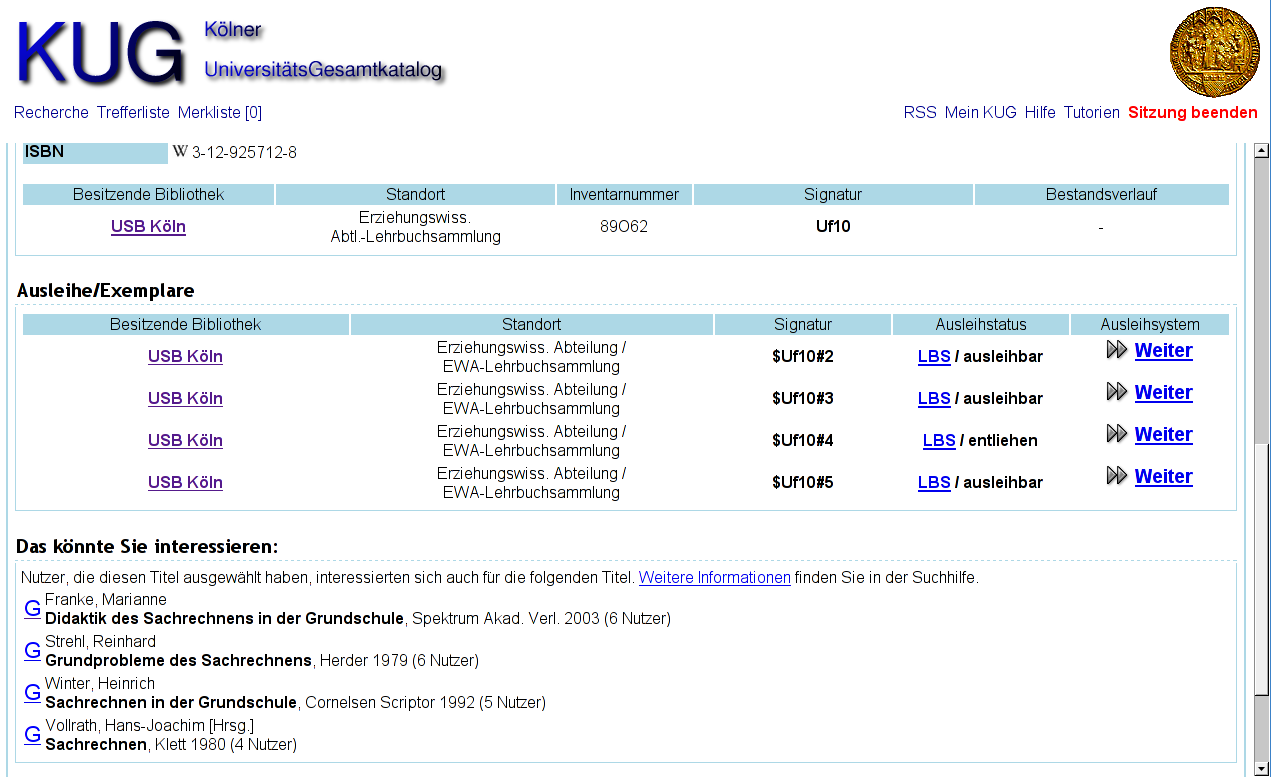
\includegraphics[width=15cm]{openbib-bfp-2007_bilder/Abb-06-recommenderfunktion.png}
    \end{minipage}
    \caption{Recommender-Informationen in der Einzeltrefferanzeige}
  \label{bild:recommender}
  \vspace{3mm}
\end{shadowenv}


Dieses Potential steckt auch in Bibliothekskatalogen und entsprechende
Funktionen können hier sinnvoll angeboten werden, wie z.B. der
Karlsruher XOPAC zeigt.

Auch OpenBib bietet solche Funktionen für den KUG an. Dazu werden
derzeit die Ausleihbewegungen sowie der Aufruf der Vollanzeige für
Titel herangezogen. Diesen Informationen werden dann entsprechende
anonymisierte Nutzer- bzw. Session-ID's zugeordnet.

Auf Grundlage der so gewonnenen Datenbasis werden im KUG folgende
Funktionen angeboten:
\begin{description}
\item[Recommender-Funktion] Zu einem konkreten Titel können andere
  Titel entsprechend des allgemeinen Nutzungsverhaltens unter der
  Überschrift "`Das könnte Sie interessieren"' (Abb.
  \ref{bild:recommender}) korreliert werden. Dazu werden
  nutzungsspezifische Überdeckungsprofile all jener anderen Titel
  erstellt, die Nutzer im Kontext des konkreten Titels angesehen bzw.
  ausgeliehen haben.
\item[Popularitäts-Informationen in Trefferlisten] Nach einer
  Recherche werden in der Trefferliste die absoluten Zugriffe anderer
  Nutzer auf die jeweiligen Titel ausgegeben. Zusätzlich kann der
  Nutzer pro Katalog bzw. katalogübergreifend nach diesen
  Popularitätsinformationen sortieren und so das Nutzungsverhalten
  anderer optional in die eigene Recherche-Strategie einbeziehen.
\item[Allgemeine Popularitäts-Informationen] Für jeden Katalog können
  weitere allgemeine Informationen angeboten werden, wie z.B. die 20
  meistgenutzten Titel usw.
\end{description}


\subsection{Drilldowns in Treffermengen}
Zur Suchverfeinerung in Treffermengen stellt OpenBib katalogweise
optional neben Tag-Clouds für die relevantesten Terme auch -- nach
Kategorien aufgeschlüsselt -- die relevantesten Kategorieinhalte dar.
Ausgehend von diesen Inhalten kann die Treffermenge über Drilldowns
weiter eingegrenzt werden. Drilldowns sind ein weit verbreitetes
Mittel, um große und unübersichtliche Treffermengen für den Nutzer zu
erschließen. OpenBib setzt diese Art von Drilldowns über
Kategorieinhalte standardmäßig daher erst bei größeren Treffermengen
ein, die aus mehr als 50 Titeln bestehen.

\subsection{RSS-Feeds}
Um den Nutzer über Neuzugänge in einem Katalog zu informieren, wurde
bewusst eine Entscheidung gegen die Implementierung herkömmlicher
E-mail-basierter Alerting-Dienste und stattdessen für den Einsatz der
sehr viel flexibleren XML-basierten RSS-Technologie
getroffen. RSS-Feeds bieten den Nutzern durch die geschickte
Verwaltung über spezialisierte Programme deutlich mehr
Nutzungsmöglichkeiten als Mails oder statische Webseiten So können
solche Programme sich um die Sichtung der Daten kümmern, schon
aufgerufene Titel von den noch nicht aufgerufenen farblich trennen,
Informationen archivieren, Data-Mining in Verbindung mit
spezialisierter Suchtechnologie einsetzen usw. Mit dieser Technik
werden seit April 2006 Neuzugangslisten der Kataloge im KUG-Kontext
angeboten. Das umfasst z.B. die letzten 50 generell in einen Katalog
aufgenommenen Titel. Ebenso lassen sich die letzten 50 Titel auch
bezogen auf einen konkreten Verfasser, eine Körperschaft, ein
Schlagwort oder eine Notation als Feed ausgehend von einer
Einzeltrefferanzeige abonnieren.

Zur Zeit werden im KUG für 113 Kataloge RSS-Feeds (Abb.
\ref{bild:rssfeeds}) angeboten. Damit nimmt die USB Köln bei dem
Einsatz dieser innovativen Technologie unter den großen
wissenschaftlichen Bibliotheken deutschlandweit eine Vorreiterrolle
ein.

\begin{shadowenv}
  \vspace{4mm}
    \centering \begin{minipage}[b]{1.0\textwidth}
      \centering 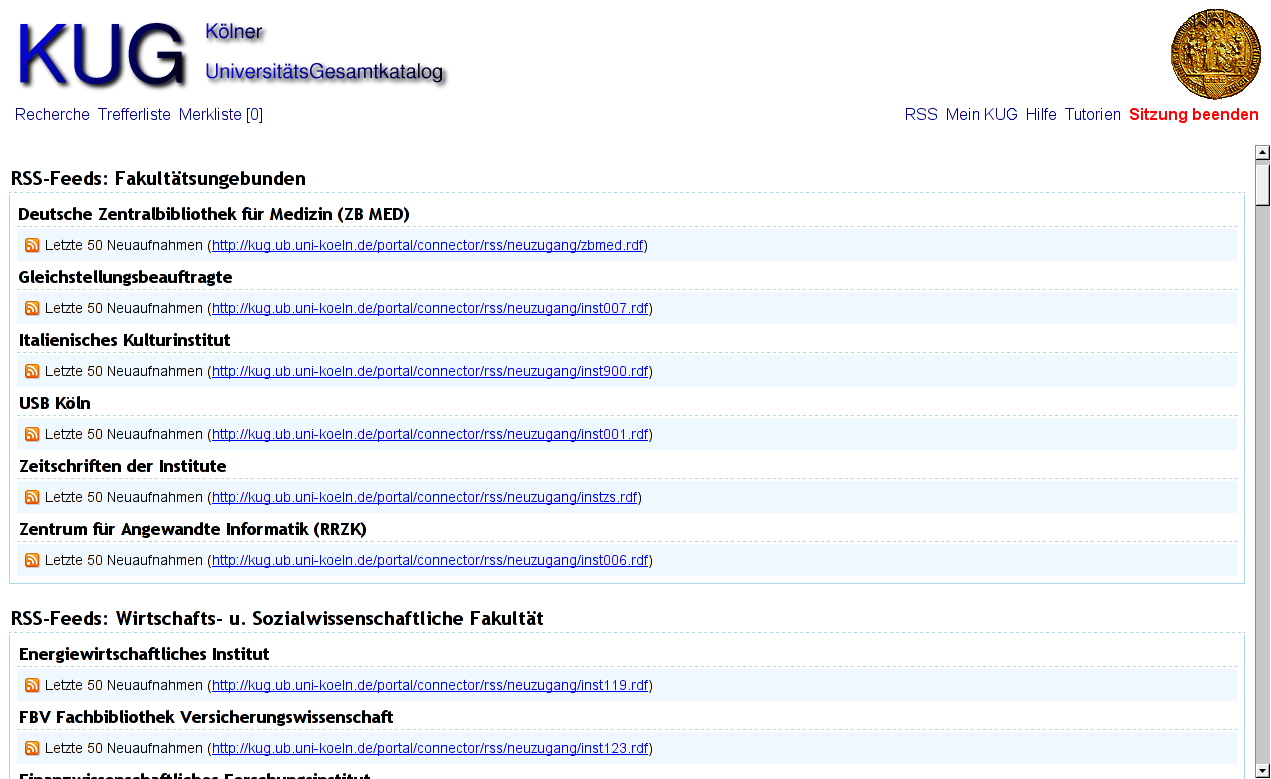
\includegraphics[width=15cm]{openbib-bfp-2007_bilder/Abb-08-rssfeeds.png}
    \end{minipage}
    \caption{Auswahl aus insgesamt 113 RSS-Feeds für Neuzugänge in den jeweiligen Katalogen des KUG}
  \label{bild:rssfeeds}
  \vspace{3mm}
\end{shadowenv}


\subsection{Mashups}
Durch die Kombination oder Integration bereits extern vorhandener
Dienste -- kurz Mashup\footnote{Artikel Mashup (Internet) aus der
  Wikipedia.\newline\path|http://de.wikipedia.org/wiki/Mashup\_(Internet)|
  (Zugriff am 30.3.2007)} genannt -- lassen sich weitere sinnvolle
Erweiterungen eines Bibliothekskataloges realisieren und dem Nutzer so
einen Mehrwert bieten.

Im KUG werden mit OpenBib verschiedene Mashups zu externen Diensten
angeboten:
\begin{description}
\item[BibSonomy] In der Einzeltreffer-Anzeige (Abb.
  \ref{bild:einzeltreffer}) wie auch in der Merkliste können die
  bibliographischen Angaben eines Titels direkt an
  BibSonomy\footnote{BibSonomy - A blue social bookmark and
    publication sharing system.\newline\path|http://www.bibsonomy.org/|
    (Zugriff am 30.3.2007)} gesendet werden. BibSonomy ist ein freier
  Social Bookmark Dienst\footnote{Entsprechend der Webseite genauer:
    Ein "`social bookmark and publication sharing system"' (Zugriff am
    30.3.2007)}, der zudem auf die Verwaltung von Bibliographie-Listen
  und deren Austausch/Verbreitung spezialisiert ist. Damit kann ein
  Nutzer direkt von dem Mehrwert profitieren, den Social-Software
  bietet und z.B. über entsprechende Tags weitere relevante Titel in
  BibSonomy finden.
\item[Wikipedia] In der Einzeltreffer-Anzeige (Abb.
  \ref{bild:einzeltreffer}) werden Personen sowie ISBNs direkt in die
  Wikipedia verlinkt. Wenn ein Nutzer Informationen zu einer Person
  oder einem Verfasser benötigt, kann er direkt eine Recherche nach
  der ensprechenden Person in der Wikipedia starten. Ebenso lässt sich
  bei vorhandener ISBN der ISBN-Suchservice der Wikipedia nutzen.
  Damit stehen dem Nutzer automatisch verschiedene Verbundkataloge,
  Buchhändler, Antiquariate usw. zur Verfügung, bei denen er direkt
  nach dem aktuell ausgewählten Titel recherchieren kann, ohne sich
  mit der jeweiligen Suchoberfläche auseinandersetzen zu müssen.
\item[DigiBib, EZB, DBIS, MedPilot] Ausgehend von einer jeden
  Recherche des Nutzers (und einer etwaigen Authentifizierung) im KUG
  kann mit Übernahme der Recherchebegriffe (und den
  Authentifizierungsinformationen im Falle der DigiBib) direkt in die
  Recherchefunktion der entsprechenden Portale gesprungen werden.
\end{description}

\begin{shadowenv}
  \vspace{4mm} \centering \begin{minipage}[b]{1.0\textwidth}
    \centering
    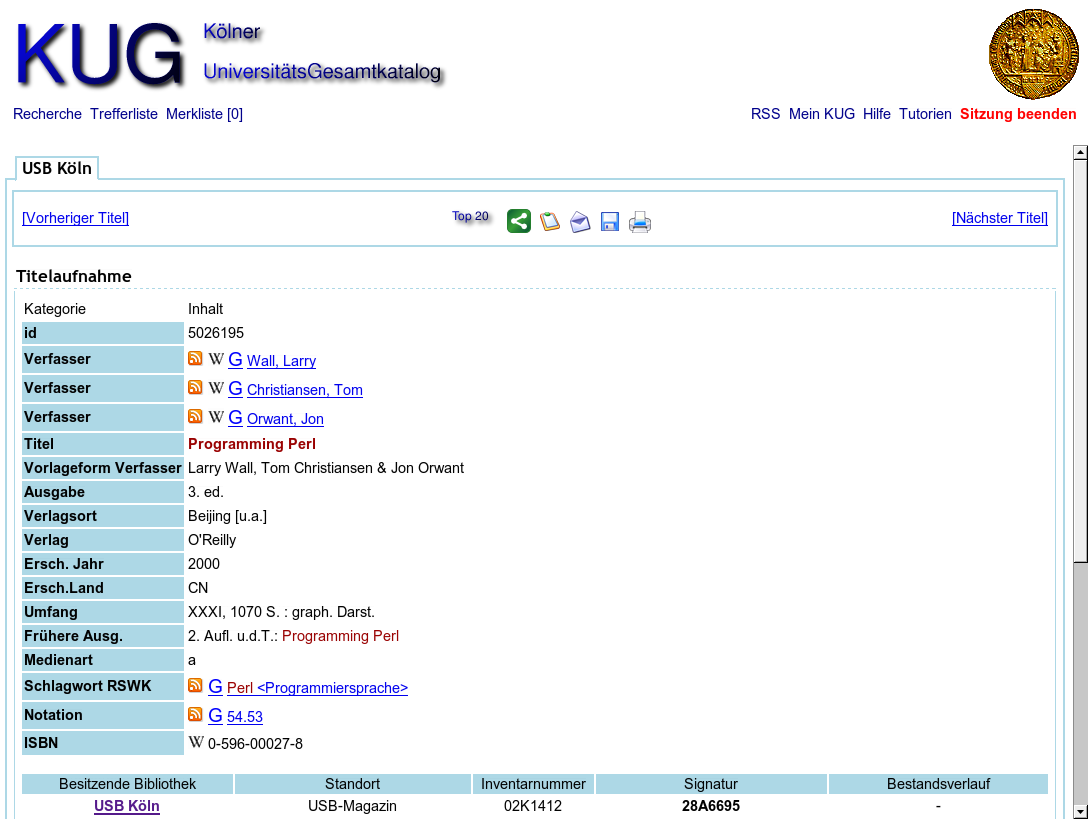
\includegraphics[width=15cm]{openbib-bfp-2007_bilder/Abb-09-mashup-einzeltreffer.png}
    \end{minipage}
    \caption{Einzeltrefferansicht mit RSS-Feeds, Mashups (Wikipedia und BibSonomy) und Suchbegriff-Highlighting}
  \label{bild:einzeltreffer}
  \vspace{3mm}
\end{shadowenv}

Umgekehrt lässt sich der KUG auch selbst (nach Absprache) über externe
webbasierte Zugriffsschnittstellen in externe Recherche-Portale über
Mashups einbinden. So sind die Bestände des KUG derzeit z.B. in die
Digitale Bibliothek NRW (DigiBib) und UK-Online\footnote{uk-online -
  Hochschul-Kommunikationssystem der Universität zu
  Köln.\newline\path|http://uk-online.uni-koeln.de/| (Zugriff am
  30.3.2007)} eingebunden.

Zur unmittelbaren Recherche im Portal über einen Web-Browser steht ein
Such-Plugin für den Browser Firefox zur Verfügung, das ausgehend von
der KUG-Hilfeseite installiert werden kann.


\section{Die Zukunft von OpenBib}
Mit den schon erreichten Funktionen von OpenBib und dem KUG ist die
Weiterentwicklung - speziell in Richtung OPAC 2.0 - noch nicht
abgeschlossen.

Für die Weiterentwicklung von OpenBib sind folgende Bereiche
vorgesehen:

\subsection{Teilhabe der Nutzer am OPAC}
Auch hier zeigen andere Online-Plattformen wie Amazon oder im
Bibliotheksbereich der Karlsruher XOPAC, wie Benutzer so eingebunden
werden können, dass sie selbst einen Mehrwert für andere Nutzer und
damit letztlich auch für die jeweilige Anwendung schaffen können. In
diesen Bereich gehören Ratings, Kommentare sowie Weiterentwicklungen
des schon vorhandenen Taggings durch Nutzer. So können z.B. ausgehend
vom Tagging-Verhalten eines einzelnen Nutzers zusätzlich
"`Nachbarschaften"' zu anderen Nutzern ermittelt und ein Zugriff auf
deren Tag-Sammlungen ermöglicht werden.

Für die so geschaffenen Informationen von Nutzern für Nutzer muss auch
überlegt werden, wie sie zwischen verschiedenen Recherche-Portalen
frei ausgetauscht bzw. generell genutzt werden können (z.B. über
WebServices). So ein Austausch würde sich auch für Informationen
anbieten, die durch dezentrale Nutzungsanalysen gewonnen werden, wie
z.B. Recommender-Informationen. Derzeit bietet die UB Karlsruhe mit
BibTip\footnote{BibTip - Ein Recommendersystem für
  Onlinekataloge.\newline\path|http://www.bibtip.de/| (Zugriff am
  13.4.2007)} bereits einen Recommenderdienst für die Integration in
externe Onlinekataloge an.

\subsection{Weitere Mashups}
Neben den bereits realisierten Mashups können weitere externe Dienste
integriert werden. Ein Beispiel in diesem Bereich ist
Geolokalisierung, wie sie schon der Dreiländerkatalog des hbz
verwirklicht. Darüber hinaus soll der Mashup mit BibSonomy dahingehend
erweitert werden, dass auch dort vergebene Tags und Verknüpfungen zu
anderen Titeln für OpenBib erschlossen werden können.

\subsection{Suchverfeinerung}
Für die Orientierung in Ergebnislisten werden in OpenBib schon
verschiedene Verfahren angewendet. In diesem Bereich soll nach
weiteren Optimierungen der bereits realisierten Drilldowns gesucht
werden. Ebenso muss analysiert werden, wie sich Klassifikationsbäume
auf Treffermengen sinnvoll einbinden lassen.

\subsection{Weitere Recherche-Backends}
Neben der Einbindung alternativer Suchmaschinen-Backends, wie
z.B. Lucene oder KinoSearch, stellt sich die Frage, wie sich
Datenbestände einbinden lassen, bei denen kein Vollzugriff auf die
Daten besteht. Hier bietet sich nur die Möglichkeit, sie über
entsprechende Abfrage-Standards wie Z39.50, SRU usw. in der Form
weiterer Recherche-Backends einzubinden. Damit fallen jedoch
automatisch auch alle bereits dargestellten Vorteile weg, die sich aus
einer einheitlichen lokalen Datenhaltung ergeben. Bei
lizenzpflichtigen Angeboten kann das aber der einzige Weg sein.

\section{Fazit}
Der KUG mit OpenBib und der neue Karslruher OPAC mit XOPAC zeigen, wie
mit Open-Source-Software innovative Wege im Bibliotheksbereich
beschritten werden können. Der Weg ist sicherlich noch weit, aber die
ersten Schritte wurden gemacht.

\newpage
\section*{Kurz-Biographie des Autors}
Oliver Flimm, Jahrgang 1969, ist Diplom-Physiker und als Administrator
sowie Programmierer im Bereich Unix/Linux seit 1991 tätig. Während
seines Studiums der Physik mit Nebenfach Informatik arbeitete er an
der USB Köln und betreute dort technisch das Projekt
InstitutsGesamtKatalog (IGK). Nach Abschluss seines Studiums übernahm
er dort als wissenschaftlicher Mitarbeiter neben seiner Tätigkeit im
Bereich Unix/Linux-Administration und -Programmierung u.a. die
technische Durchführung verschiedener Projekte -- insbesondere des
KUG-Projektes.

\section*{Anschrift des Autors}

Oliver Flimm\newline
Universitäts- und Stadtbibliothek Köln\newline
Dezernat Datenverarbeitung\newline
Universitätsstr. 33\newline
D-50931 Köln\newline
E-Mail: flimm@ub.uni-koeln.de\newline


\section*{Lizenz}

Der Artikel steht unter der Creative Commons CC-BY Lizenz

\end{document}

%%% Local Variables: 
%%% mode: latex
%%% TeX-master: t
%%% End: 
